%%%%%%%%%%%%%%%%%%%%%%%%%%%%%%%%%%%%%%%%%%%%%%%%%%%%%%%%%%%%%%%%%
% Document Class
%%%%%%%%%%%%%%%%%%%%%%%%%%%%%%%%%%%%%%%%%%%%%%%%%%%%%%%%%%%%%%%%%
\documentclass[12pt,a4paper,oneside,ngerman]{scrartcl}


%%%%%%%%%%%%%%%%%%%%%%%%%%%%%%%%%%%%%%%%%%%%%%%%%%%%%%%%%%%%%%%%%
% Packages
%%%%%%%%%%%%%%%%%%%%%%%%%%%%%%%%%%%%%%%%%%%%%%%%%%%%%%%%%%%%%%%%%
\usepackage[ngerman]{babel}
\usepackage[utf8]{inputenc}
\usepackage[nottoc,numbib]{tocbibind}
\usepackage[T1]{fontenc}
\usepackage{fancyhdr}
\usepackage{booktabs}
\usepackage[page]{totalcount}
\usepackage{tikz}
\usepackage{color, colortbl}
\usepackage{url}
\usepackage{listings}
\usepackage{tabularx}
\renewcommand{\familydefault}{\sfdefault}
\usepackage{lmodern}
\usepackage{geometry}
\usepackage{ragged2e}
\usepackage{ulem}


%%%%%%%%%%%%%%%%%%%%%%%%%%%%%%%%%%%%%%%%%%%%%%%%%%%%%%%%%%%%%%%%%
% Colors
%%%%%%%%%%%%%%%%%%%%%%%%%%%%%%%%%%%%%%%%%%%%%%%%%%%%%%%%%%%%%%%%%
\definecolor{g1}{RGB}{224,255,255}
\definecolor{g2}{RGB}{37,147,37}
\definecolor{g3}{RGB}{29,114,29}
\definecolor{g4}{RGB}{20,42,20}
\definecolor{listings}{rgb}{0.96, 0.96, 0.96}

% Java Syntaxhighligthning
% strings
\definecolor{javared}{rgb}{0.6,0,0}
% comments
\definecolor{javagreen}{rgb}{0.25,0.5,0.35}
% keywords
\definecolor{javapurple}{rgb}{0.5,0,0.35}
% javadoc
\definecolor{javadocblue}{rgb}{0.25,0.35,0.75}


%%%%%%%%%%%%%%%%%%%%%%%%%%%%%%%%%%%%%%%%%%%%%%%%%%%%%%%%%%%%%%%%%
% Page Margin
%%%%%%%%%%%%%%%%%%%%%%%%%%%%%%%%%%%%%%%%%%%%%%%%%%%%%%%%%%%%%%%%%
\geometry{
  left=2.5cm,
  right=2.5cm,
  top=2.5cm,
  bottom=2.5cm
}


%%%%%%%%%%%%%%%%%%%%%%%%%%%%%%%%%%%%%%%%%%%%%%%%%%%%%%%%%%%%%%%%%
% Definitions
%%%%%%%%%%%%%%%%%%%%%%%%%%%%%%%%%%%%%%%%%%%%%%%%%%%%%%%%%%%%%%%%%\\

\lstdefinestyle{Java}{
	language=Java,
	keywordstyle=\color{javapurple}\bfseries,
	stringstyle=\color{javared},
	commentstyle=\color{javagreen},
	morecomment=[s][\color{javadocblue}]{/**}{*/},
}

%%%%%%%%%%%%%%%%%%%%%%%%%%%%%%%%%%%%%%%%%%%%%%%%%%%%%%%%%%%%%%%%%
% Own Commands
%%%%%%%%%%%%%%%%%%%%%%%%%%%%%%%%%%%%%%%%%%%%%%%%%%%%%%%%%%%%%%%%%
\raggedright
\newcommand{\tabhvent}[1]{\noindent\parbox[c]{\hsize}{#1}}
\newcolumntype{b}{X}
\newcolumntype{s}{>{\hsize=.5\hsize}X}


%%%%%%%%%%%%%%%%%%%%%%%%%%%%%%%%%%%%%%%%%%%%%%%%%%%%%%%%%%%%%%%%%
% Document Start
%%%%%%%%%%%%%%%%%%%%%%%%%%%%%%%%%%%%%%%%%%%%%%%%%%%%%%%%%%%%%%%%%
%%%%%%%%%%%%%%%%%%%%%%%%%%%%%%%%%%%%%%%%%%%%%%%%%%%%%%%%%%%%%%%%%
% Title Page
%%%%%%%%%%%%%%%%%%%%%%%%%%%%%%%%%%%%%%%%%%%%%%%%%%%%%%%%%%%%%%%%%
\begin{document}
\thispagestyle{empty}
\vspace*{2cm}


\begin{center}
\begin{huge}
\renewcommand{\ULthickness}{2pt}
\uline{Dokumentation}
\\
\uline{Venus and Mars}
\end{huge}
\end{center}

\vspace{9cm}

\textit{\textbf{Teammitglieder: Thomas Taschner, Michael Weinberger}}
\vspace{10mm}

\textbf{{\color{g4}Version 0.5 \hfill 30.11.2015 \hfill Status: [DRAFT]}}
\\
%Table
\begin{table}[h]
\renewcommand{\arraystretch}{3.0}
\centering
\begin{tabularx}{\textwidth}{|s|s|b|b|}

\specialrule{0.07em}{0em}{0em}
\multicolumn{4}{|l|}{\textbf{Git-Pfad:} /doc/ \hfill \textbf{Dokument:} dokumentation.tex} \\ \hline
\end{tabularx}
\end{table}
\newpage


%%%%%%%%%%%%%%%%%%%%%%%%%%%%%%%%%%%%%%%%%%%%%%%%%%%%%%%%%%%%%%%%%
% Header & Footer
%%%%%%%%%%%%%%%%%%%%%%%%%%%%%%%%%%%%%%%%%%%%%%%%%%%%%%%%%%%%%%%%%
\pagestyle{fancy}
\renewcommand{\headrulewidth}{0.4pt}
\renewcommand{\footrulewidth}{0.4pt}
\setlength\headheight{15pt}
\lhead{Solarsystem}
\rhead{Version 0.5}
\lfoot{Taschner, Weinberger}
\cfoot{}
\rfoot{Seite \thepage \hspace{1pt} von \totalpages}


%%%%%%%%%%%%%%%%%%%%%%%%%%%%%%%%%%%%%%%%%%%%%%%%%%%%%%%%%%%%%%%%%
% Table of Contents
%%%%%%%%%%%%%%%%%%%%%%%%%%%%%%%%%%%%%%%%%%%%%%%%%%%%%%%%%%%%%%%%%
\tableofcontents\thispagestyle{fancy}
\newpage


%%%%%%%%%%%%%%%%%%%%%%%%%%%%%%%%%%%%%%%%%%%%%%%%%%%%%%%%%%%%%%%%%
% Changelog
%%%%%%%%%%%%%%%%%%%%%%%%%%%%%%%%%%%%%%%%%%%%%%%%%%%%%%%%%%%%%%%%%
\section{Changelog}

%Table
\begin{table}[h]
\renewcommand{\arraystretch}{3.0}
\centering
\begin{tabularx}{\textwidth}{|s|s|s|s|b|}
\hline
\rowcolor{g1} 

%Header
\tabhvent{\textbf{Version}} & \tabhvent{\textbf{Datum}} & \tabhvent{\textbf{Status}} & \tabhvent{\textbf{Bearbeiter}} & \tabhvent{\textbf{Kommentar}}  \\ \hline

%Lines
\tabhvent{\textbf{0.1}} & \tabhvent{14.10.2015} & \tabhvent{Erstellt} &  \tabhvent{Thomas Taschner} & \tabhvent{Erstellt und Inhalte hinzugefügt}         \\
\hline
\tabhvent{\textbf{0.2}} & \tabhvent{23.11.2015} & \tabhvent{Bearbeitet} &  \tabhvent{Michael Weinberger} & \tabhvent{Dokumentenstruktur geändert, Evaluierung}         \\
\hline
\tabhvent{\textbf{0.3}} & \tabhvent{24.11.2015} & \tabhvent{Bearbeitet} &  \tabhvent{Michael Weinberger} & \tabhvent{Evaluierung, Zwischenstand} \\
\hline
\tabhvent{\textbf{0.4}} & \tabhvent{24.11.2015} & \tabhvent{Bearbeitet} &  \tabhvent{Thomas Taschner} & \tabhvent{Fehlerkorrekturen} \\
\hline
\tabhvent{\textbf{0.5}} & \tabhvent{30.11.2015} & \tabhvent{Bearbeitet} &  \tabhvent{Michael Weinberger} & \tabhvent{Aktueller Zwischenstand} \\
\hline

\end{tabularx}
\end{table}
\newpage


%%%%%%%%%%%%%%%%%%%%%%%%%%%%%%%%%%%%%%%%%%%%%%%%%%%%%%%%%%%%%%%%%
% Content Start
%%%%%%%%%%%%%%%%%%%%%%%%%%%%%%%%%%%%%%%%%%%%%%%%%%%%%%%%%%%%%%%%%
\justify
%%%%%%%%%%%%%%%%%%%%%%%%%%%%%%%%%%%%%%%%%%%%%%%%%%%%%%%%%%%%%%%%%
% Übersicht
%%%%%%%%%%%%%%%%%%%%%%%%%%%%%%%%%%%%%%%%%%%%%%%%%%%%%%%%%%%%%%%%%
\section{Übersicht}
Erstelle eine einfache Animation unseres Sonnensystems!

\section{Projektbeschreibung}
\subsection{Anforderungen}
In einem Team (2 Personen) sind folgende Anforderungen zu erfüllen.

\begin{itemize}
\item Ein zentraler Stern
\item Zumindest 2 Planeten, die sich um die eigene Achse und in elliptischen Bahnen um den Zentralstern drehen
\item Ein Planet hat zumindest einen Mond, der sich zusätzlich um seinen Planeten bewegt
\item Weitere Planeten, Asteroiden, Galaxien,...
\item Zumindest ein Planet wird mit einer Textur belegt
\end{itemize}

Events:

\begin{itemize}
\item Mittels Maus kann die Kameraposition angepasst werden: Zumindest eine Überkopf-Sicht und parallel der Planentenbahnen
\item Da es sich um eine Animation handelt, kann diese auch gestoppt werden.
\item Mittels Tasten kann die Geschwindigkeit gedrosselt und beschleunigt werden.
\item Mittels Mausklick kann eine Punktlichtquelle und die Textierung ein- und ausgeschaltet werden.
\item Auch Monde und Planeten werfen Schatten.
\end{itemize}

Hinweise zu OpenGL und glut:

\begin{itemize}
\item Ein Objekt kann einfach mittels glutSolidSphere() erstellt werden.
\item Die Planten werden mittels Modelkommandos bewegt: glRotate(), glTranslate().
\item Die Kameraposition wird mittels gluLookAt() gesetzt.
\item Entfernte Objekte sollen kleiner und nahe Objekte größer.
\item Wichtig ist dabei auch eine möglichst glaubhafte Darstellung. \newline gluPerspective(), glFrustum()
\item Für das Einbetten einer Textur kann die Library Pillow verwendet werden!
\end{itemize}
\newpage
\subsection{Teammitglieder}
\begin{table}[h]
\renewcommand{\arraystretch}{3.0}
\centering
\begin{tabularx}{\textwidth}{|s|s|s|s|b|}
\hline


\tabhvent{\textbf{Name}} &\tabhvent{\textbf{Rolle}}  \\ \hline

\tabhvent{Thomas Taschner, Michael Weinberger} & \tabhvent{Entwickler, Dokumentation} \\ \hline


\end{tabularx}
\end{table}

\section{Evaluierung der Frameworks}
Im Rahmen der Evaluierung haben wir uns auf zwei Python-3D-Frameworks konzentriert, Pygame und Panda3D.
\subsection{Pygame}
Pygame ist ein plattformübergreifendes Set an Python-Modulen zur Spieleprogrammierung. Mit Millionen Downloads hat das Tool auch einen annehmbaren Verbreitungsgrad sowie eine aktive Community. Die derzeitige Version ist ausgelegt auf Python 2.7, was nicht der neuesten Version entspricht, ein inoffizieller Release verschafft Abhilfe. Wir bekamen auch den Tipp, dass die 64 Bit-Version auf manchen Rechnern schlicht nicht läuft. Außerdem fehlen wichtige, benötigte Pakete, die über pip nachinstalliert werden müssen. Das Tool an sich ist ok, jedoch ist die Usability klar verbesserungswürdig.

\subsection{Panda3D}
Panda3D ist eine kostenlose Spiele-Engine, entwickelt von Disney, der Carnegie Mellon University und einigen freiwilligen Entwicklern. Von der technischen Seite her sind viele Features vorhanden. Mithilfe der Runtime (etwa 2 MB) ist das Tool auch weitgehend plattformunabhängig, der SDK wiegt etwa 200 MB. Die gute Dokumentation, die weite Verbreitung und die vielen Beispielcodes in Foren sprechen klar für Panda3D. Die vorgefertigten Beispiele (Solar System bereits existent) sind gut aufgebaut, kommentiert und einfach erweiterbar.

\subsection{Fazit}
PyGame bietet zwar einen guten Einstieg per Video-Tutorial (in 100 Teilen, sehr zeitaufwändig), benötigt aber vom Endbenutzer eine Vielzahl an Vorbereitungen, damit das Programm ausführbar gemacht wird.

Panda3D ist unserer Ansicht nach die beste Variante die Aufgabe umzusetzen, da bereits ein entsprechendes Beispiel vorhanden ist. Die Runtime kann der Abgabe beigefügt werden inklusive Verknüpfung, so entsteht kein Aufwand für den Benutzer, da lediglich ein Doppelklick das Programm startet. \\ 
Innerhalb von wenigen Minuten ist ein zufriedenstellendes Ergebnis sehbar, die Einarbeitung und Erweiterung des Codes geht leicht von der Hand. Codebeispiele aus dem Forum/der Dokumentation können mit nur minimalen Änderungen weiterverwendet werden.
\newpage

\section{Stand vom 24. November 2015}
Das UML ist aufgrund von Panda3D und der abgenommenen Planung derzeit obsolet.
Das Example wurde angepasst, wir haben uns bereits einige Funktionen angeschaut. \\
Die Texturen wurden ausgetauscht mit höher aufgelösten, und ein Todesstern ist jetzt das Zentrum der Galaxis. Die Planetenbahnen wurden angepasst, auch der Hintergrund wurde verbessert. Als Testfall haben wir einen neuen Planeten hinzugefügt, inklusive Textur, Umlaufbahn, Größe und Rotationsverhalten. Im Hintergrund spielt der Imperial March (80\% Lautstärke, linker Audiokanal), und eine Weltraum-Kampfszene aus Star Wars als Ambiance-Musik  (100\% Lautstärke, rechter Audiokanal) \newline
Nächste wichtige Schritte:
\begin{itemize}
\item Den Code verbessern, ihn mithilfe von Designpatterns effizienter machen und aufteilen
\item Kantenglättung zum Laufen bringen
\item Bessere GUI, Navigation per Menü möglich (Overlay, Buttons?)
\item Mehr Planeten, Asteroiden, ...
\item Schatten bzw. Beleuchtung generell einbinden
\item Hilfefenster zwecks besserer Usability
\item Hintergrund verbessern bzw. Beschränkung beim Zoomen einführen
\item Nice to have: Per Klick oder Tastendruck Fokus auf bestimmten Planeten
\item Nice to have: Mehrere Galaxien (Strategy Pattern?)
\item Nice to have: Bessere Maussteuerung
\item Nice to have: Raumschiffe
\item Nice to have: Geführte Tour durchs Solarsystem, feste Routen von außen nach innen, "Ego-Perspektive"
\end{itemize}
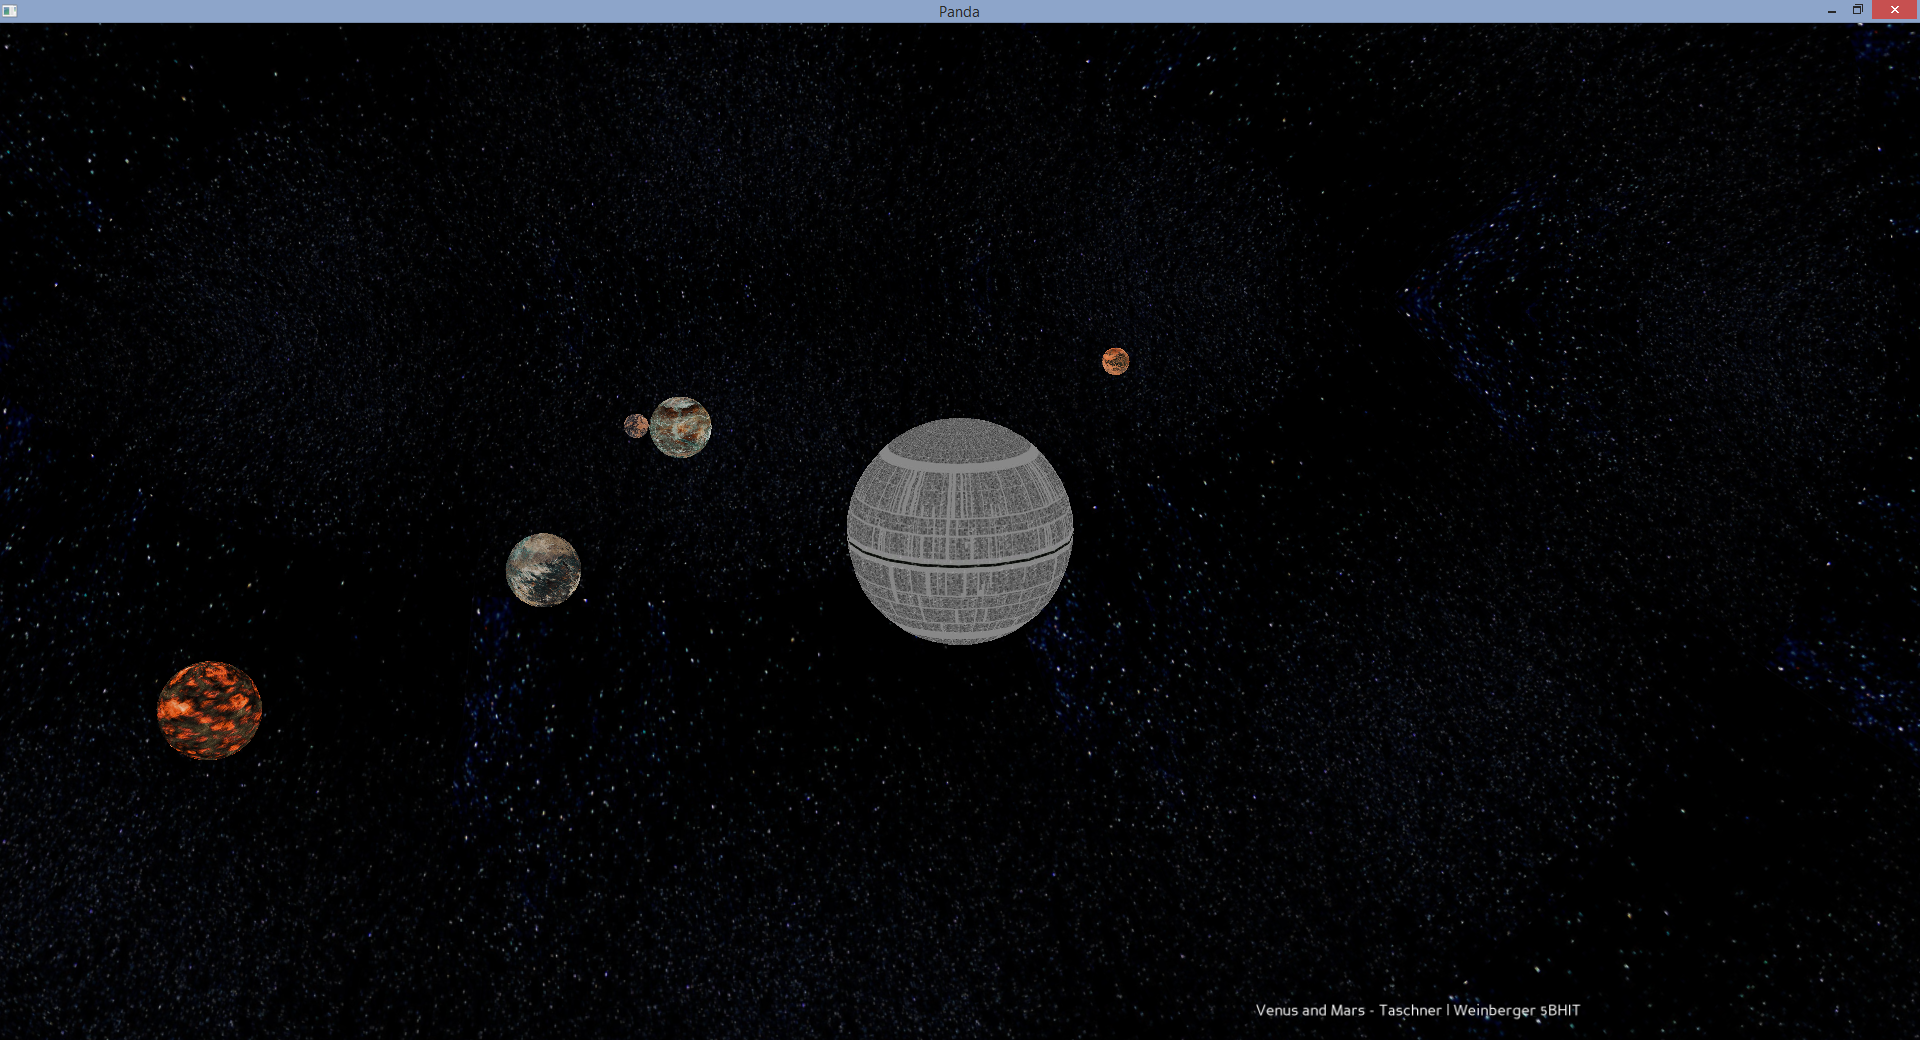
\includegraphics[width=1\textwidth]{24_11_Screen_1}
\newpage

\section{Stand vom 30. November 2015}
Im Gegensatz zur vorigen Woche hat sich vieles verändert. Da der Todesstern keine Lichtquelle ist, haben wir uns für ein DirectionalLight von der Seite entschieden. Die Kantenglättung ist noch nicht implementiert, doch aufgrund des Schattenwurfs sind diese zumindest weniger sichtbar. Mithilfe von Blender [1], einer freien 3D-Grafiksoftware, wurde von einer Modelldatenbank ein X-Wing aus Star Wars importiert. Die Software enthält Funktionen, um dreidimensionale Körper zu modellieren, sie zu texturieren, zu animieren und zu rendern. \newline \newline
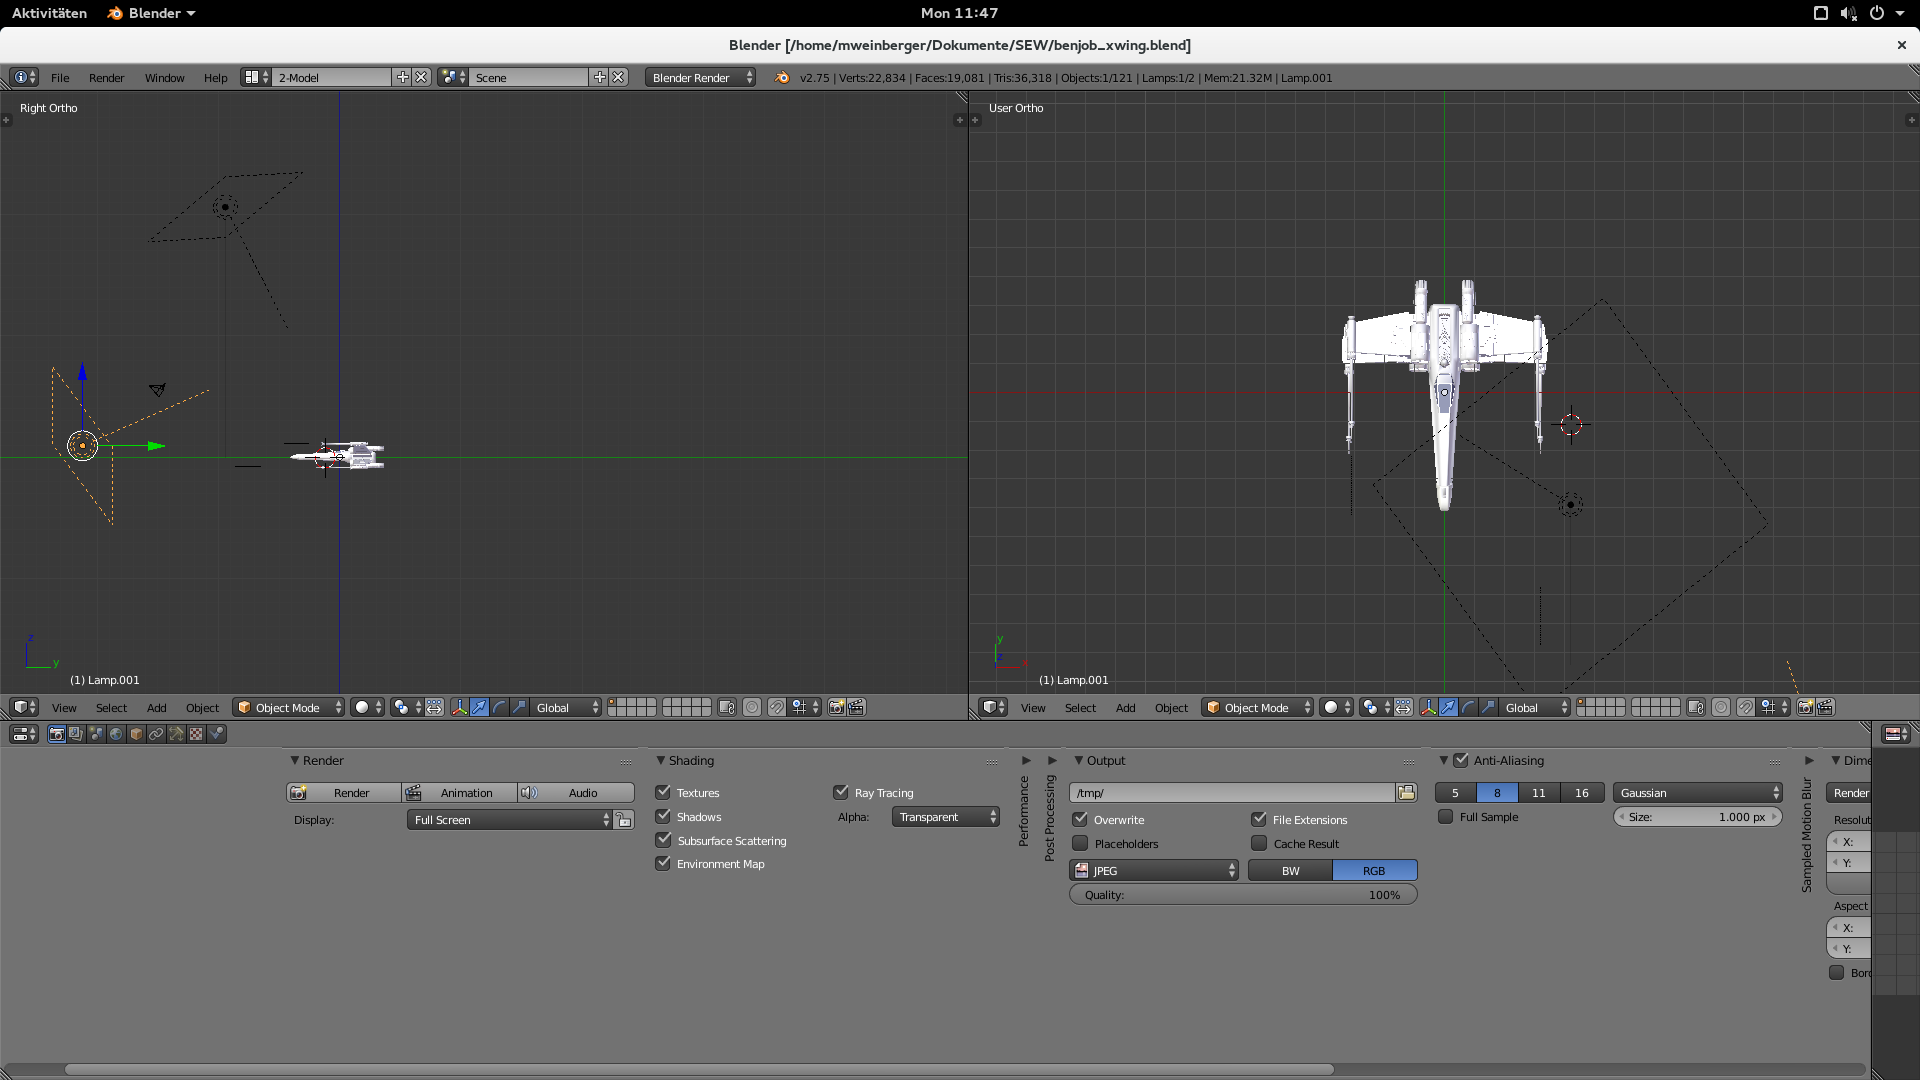
\includegraphics[width=1\textwidth]{blender_screen} \newline \newline
Der X-Wing (noch(?) ohne Textur) fliegt mit einer schnelleren Umlaufzeit als die Planeten um den Todesstern, entsprechend größenskaliert. \newline
Die Anforderungen von voriger Woche bleiben natürlich bestehen, und werden in weiterer Folge umgesetzt. \newline
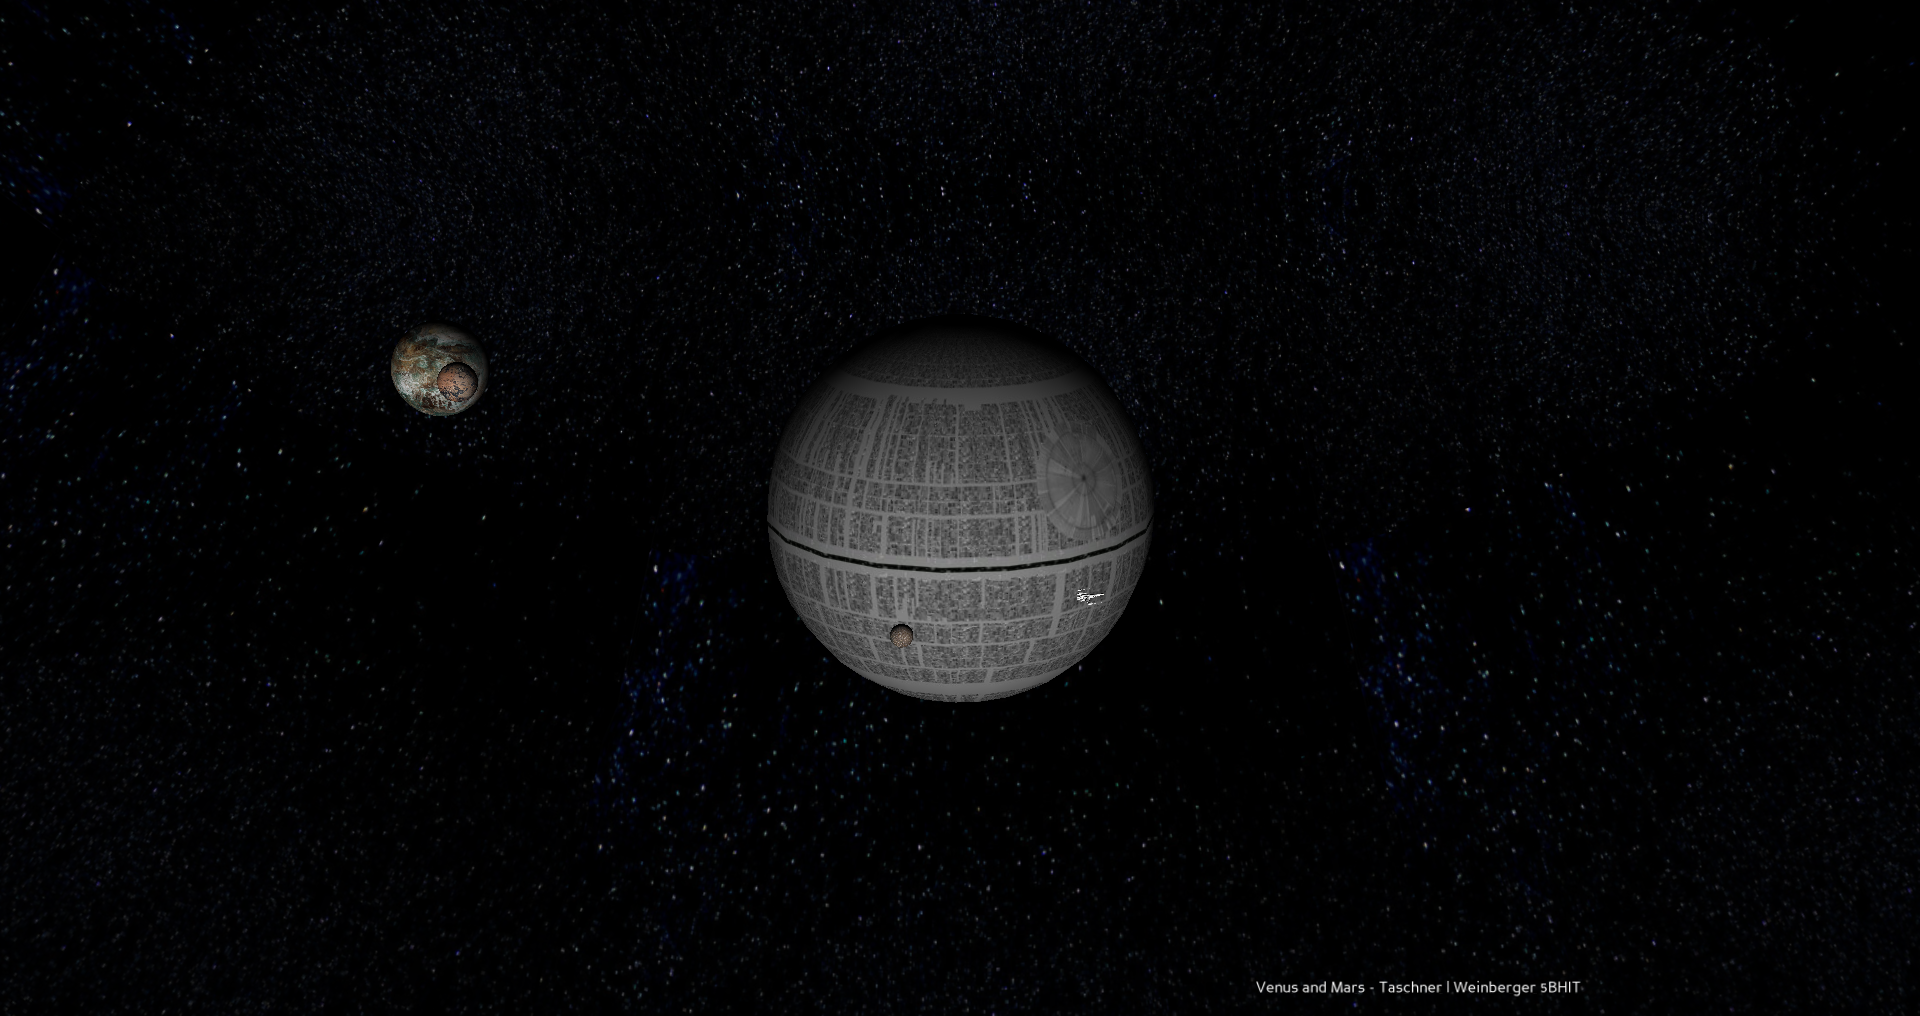
\includegraphics[width=1\textwidth]{30_11_Screen_1}
\newpage

\section{Stand vom Abgabetag 09.12.2015, Rückblick}
Ein Großteil der verbleibenden Arbeitszeit wurde für das Codedesign aufgewandt, mehr dazu in der \textit{Technischen Dokumentation}. Neben der großen Veränderung auf Codeebene wurde zuletzt noch ein Riesenplanet etwas außerhalb des gleich zu Beginn sichtbaren Planetensystems eingefügt. \newline
Der erste Punkt von 24. November, die Codeverbesserung, wurde erfolgreich abgeschlossen. Die Kantenglättung wurde obsolet, da die Treppchenbildung dank Schatten nicht mehr sichtbar war. Die Entwicklung einer umfangreicheren GUI wurde zwecks Ressourcenoptimierung ausgesetzt, dafür haben es mehr Planeten ins fertige Programm geschafft. Da der Todesstern keine Lichtquelle ist, wurde eine Beleuchtung von der Seite aus implementiert. Bei der Problematik des Hintergrunds (Ende des Bereichs sichtbar bei zu großem Zoom) wurde auch eine Lösung gefunden: Die Galaxie-Sphere um den Faktor 10 größer machen, nun ist beim Zoom diese harte Grenze um einiges schwieriger zu erreichen. \newline \newline
\textbf{Damit das Programm ausgeführt werden kann, muss die Panda3D-Runtime installiert werden.} \newline
Über eine Verknüpfung mit der Runtime, unter Windows etwa \textit{D:/Programme/Panda3D-1.8.1/python/python.exe -E VenusAndMars.py}, kann das Programm dann gestartet werden.


\newpage

%%%%%%%%%%%%%%%%%%%%%%%%%%%%%%%%%%%%%%%%%%%%%%%%%%%%%%%%%%%%%%%%%
% Quellen
%%%%%%%%%%%%%%%%%%%%%%%%%%%%%%%%%%%%%%%%%%%%%%%%%%%%%%%%%%%%%%%%%
\section{Quellen}
[1]: https://www.blender.org/, Blender Foundation, zuletzt abgerufen am 30.11.2015 \newline

%%%%%%%%%%%%%%%%%%%%%%%%%%%%%%%%%%%%%%%%%%%%%%%%%%%%%%%%%%%%%%%%%
% Content End
%%%%%%%%%%%%%%%%%%%%%%%%%%%%%%%%%%%%%%%%%%%%%%%%%%%%%%%%%%%%%%%%%
\end{document}
%%%%%%%%%%%%%%%%%%%%%%%%%%%%%%%%%%%%%%%%%%%%%%%%%%%%%%%%%%%%%%%%%
% Document End
%%%%%%%%%%%%%%%%%%%%%%%%%%%%%%%%%%%%%%%%%%%%%%%%%%%%%%%%%%%%%%%%%